\chapter{算法实现}
本章,我们将从判决预测、关键词抽取、类案搜索等模块来详细介绍项目中用到的算法模型。在模型中,我们统一使用了THULAC进行中文分词,我们使用的词向量是利用FastText模型,在大规模的法律文书语料库上进行的预训练,我们采用的词向量维度为200维。

对于每一个模块,我们将分别从任务的描述定义、算法的创新点、算法模型细节三个方面来进行详细阐述。

\section{背景知识}
\subsection{卷积神经网络}
卷积神经网络(Convolutional Neural Network, CNN)是一种前馈神经网络,它的人工神经元可以响应一部分覆盖范围内的周围单元,对于大型图像、文字等处理有出色表现。

卷积神经网络通常包含以下结构:

\begin{itemize}
	\item \textbf{卷积层(Convolutional layer)}:卷积神经网路中每层卷积层由若干卷积单元组成,每个卷积单元的参数都是经过\textbf{反向传播算法}训练得到的。卷积运算的目的是提取输入的不同特征。
	\item \textbf{线性整流层(Rectified Linear Units layer, ReLU layer)}:使用线性整流作为激活函数。它可以增强判定函数和整个神经网络的非线性特性,而本身并不会改变卷积层。
	\item \textbf{池化层(Pooling layer)}:通常在卷积层之后会得到维度很大的特征,将特征切成几个区域,取其最大值或平均值,得到新的、维度较小的特征。
	\item \textbf{全连接层(Fully-Connected layer)}:完成从输入到标签集的映射,即分类。
\end{itemize}

\begin{figure*}[h]
    \centering
    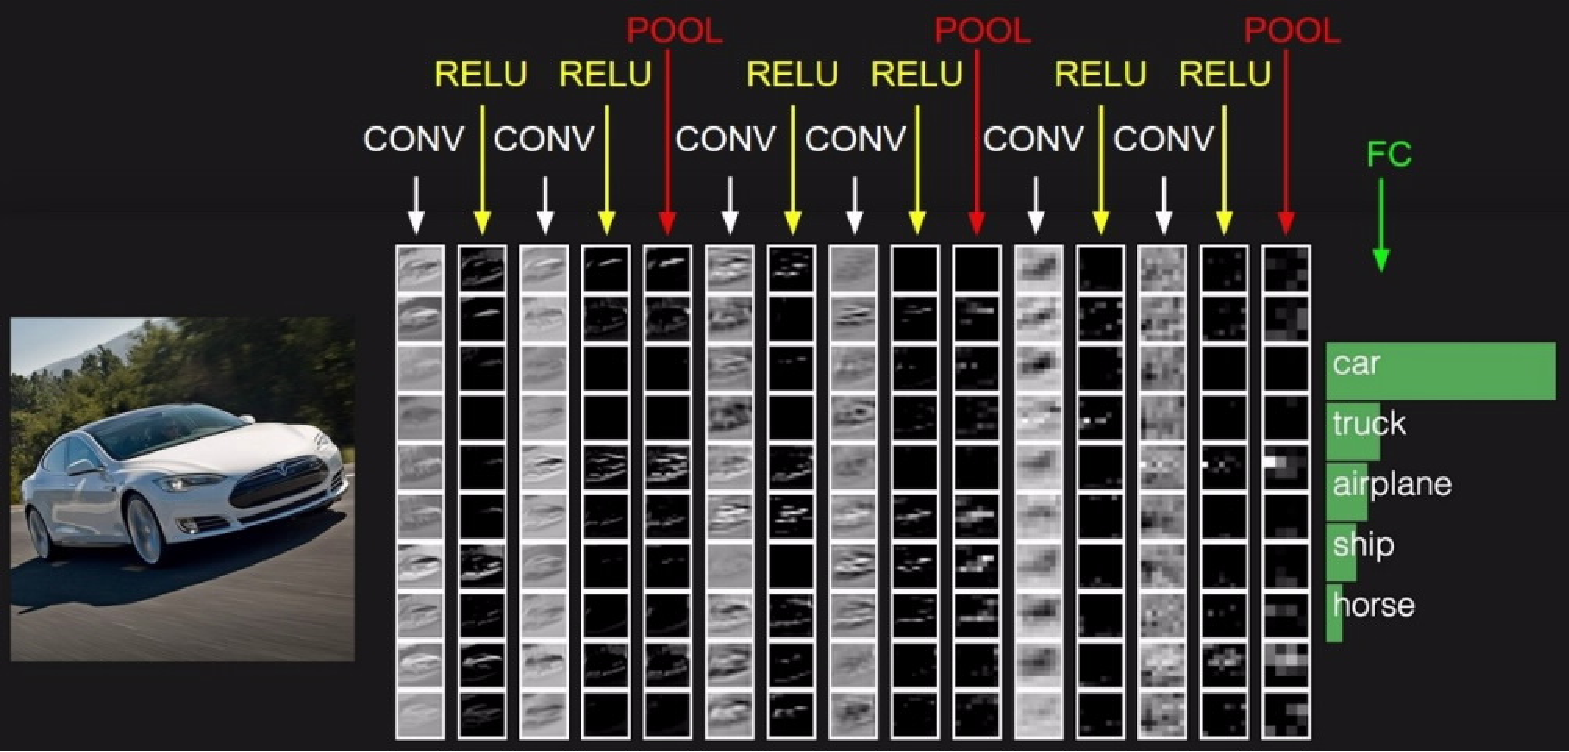
\includegraphics[width=\linewidth]{figures/cnn1}
    \caption{卷积神经网络实例}
    \label{fig:cnn1}
\end{figure*}

图~\ref{fig:cnn1}是一个卷积神经网络各层应用的实例:


卷积神经网络中最基础的操作是卷积。基础 CNN 所用的卷积是一种 2-D 卷积。也就是说,卷积核(kernal)只能在 x,y 上滑动位移,不能进行深度(跨通道)位移。

卷积需要输入两个参数,实质是二维空间滤波,滤波的性质与卷积核选择有关,CNN 的卷积是在一个 2-D 卷积核与 2-D 输入映射之间,在各通道分别完成的。

我们假设单一通道输入的空间坐标为 ${\displaystyle (x,y)}$,kernel 大小是 ${\displaystyle p \times q}$,kernel 权重为 ${\displaystyle w}$,图像亮度值是 ${\displaystyle v}$,卷积过程就是 kernel 所有权重与其在输入图像上对应元素亮度之和,可以表示为:${\displaystyle conv_{x,y} = \sum_i^{p*q}w_i v_i}$。

下面即是一个例子:

\begin{figure*}[ht]
    \centering
    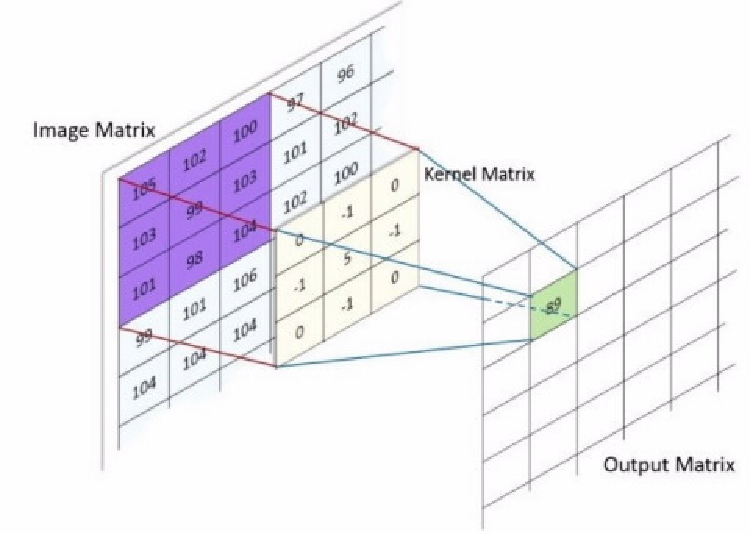
\includegraphics[width=\linewidth]{figures/cnn_conv}
    \caption{卷积层的例子}
    \label{fig:cnn_conv}
\end{figure*}

将 kernel 随 ${\displaystyle (x,y)}$ 平移扫描,即可以得到输出空间。需要特别说明的是,卷积层可能包含多个 kernel,用以抓取多个特征;扫描步长、方向也可能有所不同。

卷积之后,通常会加入偏置(bias),并引入非线性激活函数(activation function),令偏置为 ${\displaystyle b}$,激活函数为 ${\displaystyle h\left(\right)}$,经过激活函数后,得到的结果是 ${\displaystyle z_{x,y}=h\left(\sum_i^{p*q} w_i v_i +b\right)}$。

池化(Pooling)是卷积神经网络中另一个重要的概念,它实际上是一种形式的降采样。有多种不同形式的非线性池化函数,而其中“最大池化(Max pooling)”是最为常见的。它是将输入的图像划分为若干个矩形区域,对每个子区域输出最大值。直觉上,这种机制能够有效地原因在于,在发现一个特征之后,它的精确位置远不及它和其他特征的相对位置的关系重要。池化层会不断地减小数据的空间大小,因此参数的数量和计算量也会下降,这在一定程度上也控制了过拟合。通常来说,CNN 的卷积层之间都会周期性地插入池化层。

池化层通常会分别作用于每个输入的特征并减小其大小。目前最常用形式的池化层是每隔 2 个元素从图像划分出 ${\displaystyle 2\times 2}$ 的区块,然后对每个区块中的 4 个数取最大值。这将会减少 75\% 的数据量。

出现在 CNN 最后的全连接层的主要目的是分类。这与神经网络中的全连接层是相同的。

CNN 网络的训练一般使用反向传播(Back Propagation)算法。同样地,这即是传统神经网络训练的常用算法。


\subsection{长短时记忆网络}

长短时记忆网络(Long short-term memory, LSTM)是一种用于深度学习领域的循环神经网络(Recurrent Neural Network, RNN)架构。与其他神经网络架构不同,LSTM 网络非常适合基于时间序列数据进行分类、处理和预测。

循环神经网络相比全连接神经网络更擅长处理序列数据,与传统神经网络不同,它们是具有循环的网络,这将允许信息持续存在。

咕咕咕,这里有一张图

上图是一个示意图,一组神经网络 A 接收某些输入 ${\displaystyle x_t}$,并输出一个值 ${\displaystyle h_t}$。循环允许信息从网络的一个步骤传递到下一个。

RNN 的重要能力在于它可以将以前的信息连接到当前任务,例如使用先前的视频帧来帮助对当前帧的理解。然而,对于较长距离的历史信息,RNN 仍无法有效地将其利用。

LSTM 相对 RNN 而言解决了长依赖关系学习的问题,能够记住长时间间隔内的信息。通常地,一个 LSTM 单元包含细胞、输入门、输出门和忘记门。其中,细胞(用${\displaystyle C_t}$ 表示)用于记录需要的长时间间隔的信息;输入门、输出门、忘记门具有删除或添加信息到细胞状态的能力,它们被用于维护细胞的状态、控制进出单元的信息流。

下图是一个示意图:

咕咕咕,这里有另一张图


\subsection{条件随机场}


\section{判决预测}
\subsection{任务描述}
司法的一个重要作用便是对现实生活中发生的各类纠纷、案例以及违法法律的情况进行裁决,而判决就是体现这个裁决的重要场景,而判决结果是每一个案件最关键的基础特征,为了能够直观地捕获到案件的核心特征,在该模块中,\textbf{我们实现了对法学判案要素预测、案件的罪名/案由判断、相关法条推荐、量刑预测功能}。

这四个任务的结果之间具有很强的前后依赖关系,例如,最终量刑强烈依赖于法条的相关规定。在该模块中,四个任务按照顺序构成任务序列,分别对应于模型中$task_{1}$至$task_{4}$。

输入一段文本形式的案情描述,模型通过阅读文本获取其中蕴含的语义信息,将案情映射到高维向量空间,得到一个蕴含关键判案信息的文章向量。在该模块中,我们应用了多任务学习模型(multi-task learning),利用相同的编码器捕获文本信息,通过对每一个任务设置不同的输出层,将高维文本向量映射到不同的输出结果之上。
%再根据不同的任务,将文章向量喂给不同的输出层获得不同的分类结果。

\begin{figure*}[ht]
    \centering
    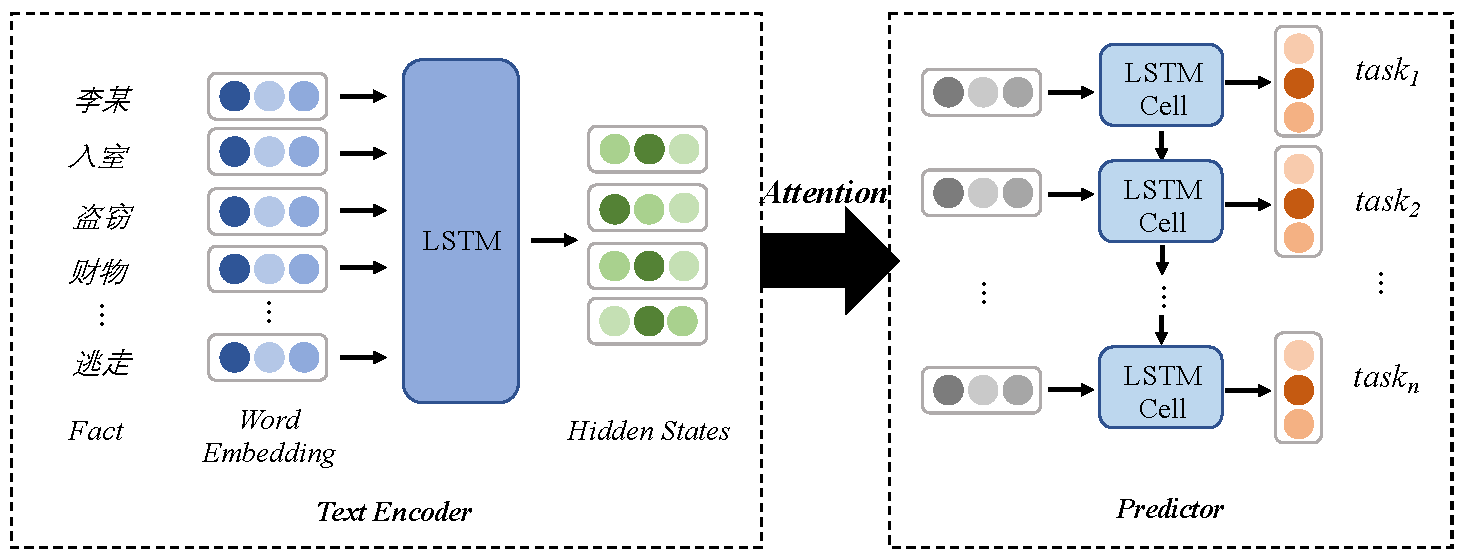
\includegraphics[width=\linewidth]{figures/model1}
    \caption{判决预测模型示意图}
    \label{fig:model1}
\end{figure*}

\subsection{创新点}
我们将上述问题总结为文本分类问题,然而由于无法考虑到在实际法律场景运用中的数据不均衡、相似罪名难以区分等问题,传统文本分类模型在这些任务上无法取得令人满意的效果。通过观察基线模型的预测效果,我们发现了以下现有模型无法解决的难点:
\begin{itemize}
	\item \textbf{数据不均衡(Few-shot)}。在实际场景数据集中,不同案由的案件数量具有极度不均衡性。根据我们对裁判文书网上刑事案件的统计,实际生活中遇到的案件,最频繁发生的十类案件数量(例,盗窃案件、故意伤害案件等)达到了总案件数量的$78.1\%$,然而与此正相反,频率最低的50个罪名案件数量(例,扰乱法庭案、逃税案)只占案件总数量的不到$0.5\%$。以往模型往往关注在高频案件,而忽略了低频案件的判决,然而低频罪名的判决恰恰需要更加大量的法律专业知识。低频罪名的判断也成为提高判决系统稳定性、实用性的关键所在。
	\item \textbf{易混淆罪名难以辨析}。在我国法律体系中存在很多相似的易混淆罪名(例如,盗窃与转化型抢劫、挪用公款罪与贪污罪)。细微的事实改变就可以改变被告罪名判决结果,以往模型在这些罪名上将出现大量的混淆。
	\item \textbf{预测结果矛盾}。传统模型在预测多个任务时,往往因为无法正确捕捉任务之间的依赖关系而预测出矛盾的结果。以往模型往往会预测出完全无关的相关法条、罪名与刑期等,例如模型预测被告为盗窃罪,在刑期上却预测出死刑。预测结果的矛盾导致了以往模型无法运用到实际。
\end{itemize}

在此基础上,我们提出了一个新的判决预测模型,该模型能够捕捉到不同任务之间前后依赖关系,同时通过模拟人类法官判案思路,将判断案件法学要素作为预测判决结果的子任务来提升模型在混淆罪名与低频罪名上的预测效果。综上,我们做出了以下贡献:
% 我们将上述所有功能归纳为文本分类问题,通过观察,上述任务之间有很强的前后依赖关系,例如,相关法条推荐结果往往与罪名及案由预测结果高度相关。并且,根据法学领域从业人员介绍,在实际判案时,大家首先会判断案情中的相关要素,并根据要素判断结果来决定最后的案件的判决。因此,我们有以下创新来提升各个任务的效果:

\begin{itemize}
	\item 提出了一个新的具有高度可扩展性的多任务学习(multi-task learning)模型,相比于以往多任务学习模型,我们的模型可以充分利用各个任务之间的依赖关系,避免了不同任务之间预测结果的矛盾性,同时提升了模型在多个任务的预测效果。
	\item 提出了判决预测新的子任务——判案要素预测,模型通过预测不同案件之间共有的法学要素,来提升模型对法律案件的特征抽取能力。在低频案件的预测上,相比于基线模型,我们的模型实现了超过50\%的效果提升。我们采用了10个最常见的判案要素,如表格\ref{tab:key_elements}所示,要素判断结果可以很好地帮助我们对案件被告涉及罪名做出判断。
	\end{itemize}

\begin{table}[]
\center
\begin{tabular}{l|l}
\hline
\textbf{要素}          & \textbf{要素描述}   \\ \hline
盈利          & 被告犯罪是否以盈利为目的       \\
买卖          & 被告行为中是否涉及买卖行为      \\
死亡          & 被害人是否死亡            \\
暴力          & 被告是否采用了暴力手段犯罪      \\
国家机关/国家工作人员 & 案件中是否涉及国家机关与国家工作人员 \\
公共场合        & 案件是否发生在公共场合        \\
非法占用        & 被告是否以非法占用为目的       \\
伤害          & 被害人是否受伤            \\
主观故意        & 被告主观上是否故意犯罪        \\
生产作业期间      & 案件是否发生在生产作业期间  \\ \hline   
\end{tabular}
\label{tab:key_elements}
\caption{判案要素表}
\end{table}


\subsection{算法模型}
% 算法使用了LSTM作为模型的编码器,使用了全连接神经网络作为输出层。利用了多任务学习的框架,将多个任务进行联合训练得到了效果的提升。
输入案情文本描述后,我们将其进行分词操作将案情描述划分为词语序列$x = \{x_{1}, x_{2}, ..., x_{n}\}$,其中$n$为词语数量。同时,模型适用于multi-task learning任务,我们假设有案件预测结果为$T$,其中$Y = \{y_{1}, y_{2}, ..., y_{|T|}\}$,$y_{i}$为第$i$个子任务的结果。

在该模型中,我们利用长短时记忆网络(LSTM)作为文本编码器,生成案情文本的表示向量。LSTM是循环神经网络的一个变种,通过在每一个循环单元引入输入门、遗忘门、输出门和记忆单元来帮助神经网络捕捉长序列的信息。考虑到我们的输入文本较长,为了捕捉长文本序列关系,我们采用了LSTM作为编码器。编码器结构可分成以下几层。
\begin{itemize}
	\item \textbf{输入层}:文本分词与词向量映射。在获取到输入文本后,我们采用了THULAC作为文本分词器对文本进行分词,同时我们采用了FastText模型在数据集上预训练了词向量。在本层,通过查词向量表,我们将每一个输入单词$x_{i}$转换成词向量$\mathbf{x}_{i}$。此时,输入的文本已经被转换成
	\begin{equation}
		\hat{x} = \{\mathbf{x}_{1}, \mathbf{x}_{2}, ..., \mathbf{x}_{n}\}
	\end{equation}
	\item \textbf{编码层}:为了能够让捕捉到词语序列前后文信息,我们用LSTM对获取到的词向量进行编码处理,获得隐向量序列$\mathbf{h} = \{\mathbf{h}_{1}, \mathbf{h}_{2}, ...,\mathbf{h}_{n}\}$。其中
		\begin{equation}
			\mathbf{h}_{i} = LstmCell(\mathbf{x}_{i}, \mathbf{h}_{i-1})
		\end{equation}
	\item \textbf{注意力层}:我们在循环神经网络基础之上运用了注意力机制(attention)捕获输入文本中的关键信息。通过attention机制,我们可以根据任务的不同,捕获到不同的关键信息,从而为每一个任务都生成一个不同的表示向量$\mathbf{a} = \{\mathbf{a}_{1}, \mathbf{a}_{2}, ..., \mathbf{a}_{n}\}$。其中,$\mathbf{u}^{k}$为每个子任务的表示向量,$\mathbf{W}^{a}$为训练参数。
		\begin{equation}
			\mathbf{a}_{i} = \sum_{j=1}^{n}\alpha_{j}\mathbf{h}_{j}
		\end{equation}
		\begin{equation}
			\alpha_{j} = \frac{exp(tanh(\mathbf{W}^{a}\mathbf{h}_{j})^{T}\mathbf{u}^{k})}{\sum_{t}exp(tanh(\mathbf{W}^{a}\mathbf{h}_{t})^{T}\mathbf{u}^{k})}
		\end{equation}
	\item \textbf{预测层}:在为每一个任务获得其表示向量后,我们利用了LSTM Cell捕捉长序列信息的能力来获取前后任务之间的依赖关系。我们将Attention层的输出当做预测层的输入序列,为每一个子任务初始化一个不同的LSTM单元,从而获取与任务相关的文本表示向量$\hat{\mathbf{ht}}_{i}$。
		\begin{equation}
			\hat{\mathbf{ht}}_{i} = LstmCell(\mathbf{a}_{i}, \mathbf{ht}_{i})
		\end{equation}
		\begin{equation}
			\mathbf{ht}_{i} = \mathbf{W}_{i}\mathbf{ht}_{i-1} + \mathbf{b}_{i}
		\end{equation}
	\item \textbf{输出层}:最后,在获得每一个任务特有的文本表示向量之后,我们采用了全连接神经网络,将包含任务信息的文本向量映射到每个任务相应的分类中。对于每个不同的任务而言,$\mathbf{y}_{i} \in \mathbf{Y}_{i}$,其中$\mathbf{Y}_{i}$是每个任务的分类空间,例如对于罪名预测任务而言,$Y =$\{盗窃罪、抢劫罪……\}
		\begin{equation}
			\mathbf{y}_{i} = softmax(\mathbf{\hat{W}}_{i}\mathbf{ht}_{i} + \mathbf{\hat{b}}_{i})
		\end{equation}
	
\end{itemize}

我们采用了交叉熵损失函数,运用了Adam算法训练模型参数。其中损失函数计算公式如下,
\begin{equation}
	\mathcal{L} = \sum_{j}\mathcal{L}_{j}
\end{equation}
\begin{equation}
	\mathcal{L}_{j}(\hat{\mathbf{y}_{j}}, \mathbf{y}_{j}) = -\sum_{k=1}^{|Y_{j}|}\mathbf{y}_{j, k}log(\hat{\mathbf{y, k}})
\end{equation}

我们将算法运用于判案要素预测、罪名预测、法条预测、刑期预测四个任务上,四个任务的预测结果前后依赖,罪名预测结果依赖于要素预测结果,刑期预测结果与法条内容高度相关。因此,我们将四个任务按照上述顺序构成任务序列,利用任务之间的相关关系,提升各个任务的效果。具体实验结果见章节\ref{cha:result}。


\section{关键词抽取}
\subsection{任务描述}
关键词抽取是自然语言处理领域的传统任务,但是传统的基于词频、词性特征的关键词抽取算法,需要大量的人工介入,不具有良好的扩展性。因此,我们提出了在法律领域的关键词抽取,我们利用了神经序列标注模型对案情文本中每一个词进行标注。任务输入为一段案情描述的文本,任务的输出为文本中的某一个或者某一些关键词语,这些词语作为文本的法律标签,是用来检索相关案件、法条的重要依据。

我们将关键词定义为文本中可以帮助检索相关案件、相关法条的词语。例如,对于句子:“被告对{\color{red}火灾}发生是否存在{\color{red}过错},应否对原告的合理损失予以{\color{red}赔偿}”中标红的即为关键词,这些关键词可以很好地帮助检索相关法律法规:“关于{\color{red}火灾过错}引发事故责任划分与{\color{red}赔偿}…”。

本模块我们采用了对句子级别的预料进行训练的方式,我们整理了10000条待标注数据,通过寻找专业人士进行人工标注的方法,获取了相应的待标注的训练数据。

在使用时,我们将对每一个句子进行关键词抽取,筛除其中逆文本频率低的词语,将所有句子的关键词进行合并、筛选,得到最终文章级别的关键词。关键词抽取的结果将对后续的相关案例检索提供重要的帮助。

\subsection{创新点}

关键词抽取是自然语言处理中。在早期,大多数人们使用的是基于词频等特征的无监督学习算法,例如TextRank、LDA、TFIDF算法。对于法律这样一个特定领域,关键词抽取的结果往往是一些法言法语,相比于开放领域上的关键词抽取,有着更强的规律性。因此,我们将目前效果最好的命名实体识别算法运用至该任务。同时,由于训练是在句子级别的语料上进行训练,我们设计了筛选算法,将在所有句子上的抽取结果进行合并筛选,得到了一个较好的效果。

\subsection{算法模型}

\begin{figure*}[ht]
    \centering
    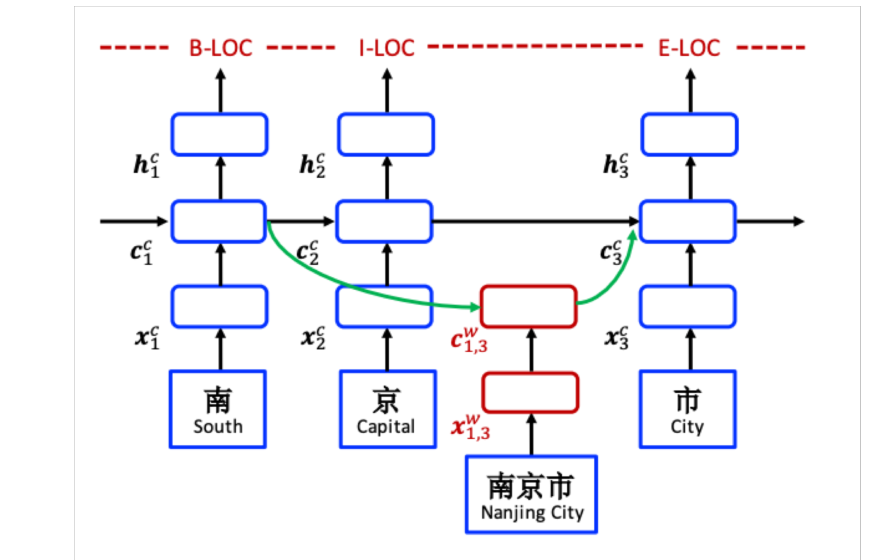
\includegraphics[width=\linewidth]{figures/model2}
    \caption{关键词抽取模型示意图}
    \label{fig:model2}
\end{figure*}

该算法将目前前沿的命名实体识别算法——Lattice LSTM,通过将句子拆分成字级别,对每一个字一个标签,来判断最终关键词的范围。在传统的基于字级别的模型基础上,加入词级别信息,这样克服了字级别信息不足、词级别过度依赖于分词效果的缺陷。

1)	利用n-gram、分词信息等特征为句子中每一个字进行编码,形成字级别特征;

2)	利用好BiLSTM-CRF的框架,通过BiLSTM对字特征进行编码,再通过CRF捕捉序列信息,进行序列标注;

3)	改造字级别的LSTM模型,将字与字之间匹配成的所有的可能词的特征融合到LSTM的信息传递中,得到一个Lattice-word model;

4)	对每个字预测BIE标签,其中B为begin、I为in、E为end;得到最后序列标注的结果。



\section{类案搜索}
\subsection{任务描述}
该模块实现了相关案例推荐的功能。该功能的实现主要基于上述两个模块的模型。该任务模型以案情描述作为输入,通过关键词标签抽取,检索到一批与该案情相似的法律文书,再利用判决预测模块得到的文本向量,对检索到的文书进行重排序,输出一个按照相似度递减的法律文书集合。

\subsection{创新点}
该任务所用算法与传统的搜索引擎算法不同,传统搜索引擎将检索文本与数据库文本进行比对,进而检索出相似度高的文本段。在我们算法中,我们通过抽取出的关键词标签来初步确定相关的文章的集合,再通过判决预测模块中获得的包含文本语义的向量,来对相关集合进行重排序,得到在语义层面相似度最高的文章。

这样的做法改善了传统搜索引擎只关注文本相似度的缺点,通过捕捉语义信息检索以满足用户需求。

\subsection{算法模型}
如上所述,改算法主要分成以下两步:

1)	抽取关键词,利用关键词抽取模块将案情描述中的关键词抽取出来。

2)	利用关键词标签,确定相关文书的集合;将所有关键词与该案情描述关键词一样的案件抽取出来,形成相关文书集合。

3)	相关程度重排序,利用判决预测模块将第2步获得的文书,转化成包含语义信息的文本向量,通过向量的距离来判断文书与输入案情的相关程度,按照相关程度对文书进行重排序。



